\section{Nonlinear Vector Auto-Regression}

\vspace{1em}
\begin{minipage}{\textwidth}
    \centering
    \begin{tikzpicture}[scale=1]

        % --- State vectors
        \node(tm1) at (-12, 6){
            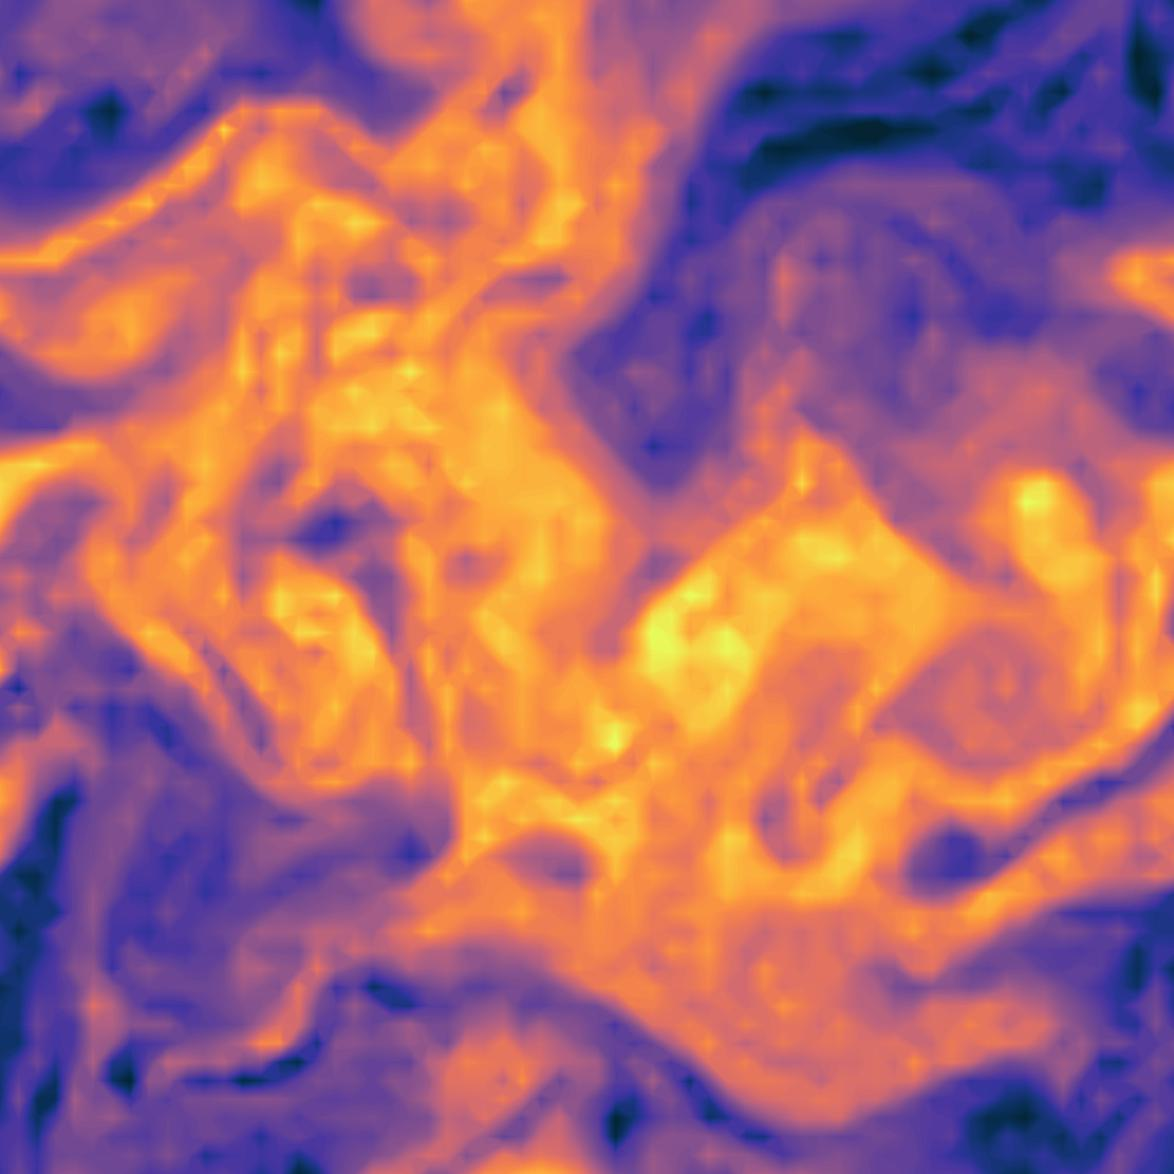
\includegraphics[width=.22\textwidth]{../../figures/theta-t-1.jpg}
        };
        \node at
            ($ (tm1.north) + (0.0, 0.5) $)
            {$\inputstate(t-N_\text{lag})$};

        \node at (-6, 6) {$\bullet\,\,\bullet\,\,\bullet$};

        \node(t0) at (0, 6){
            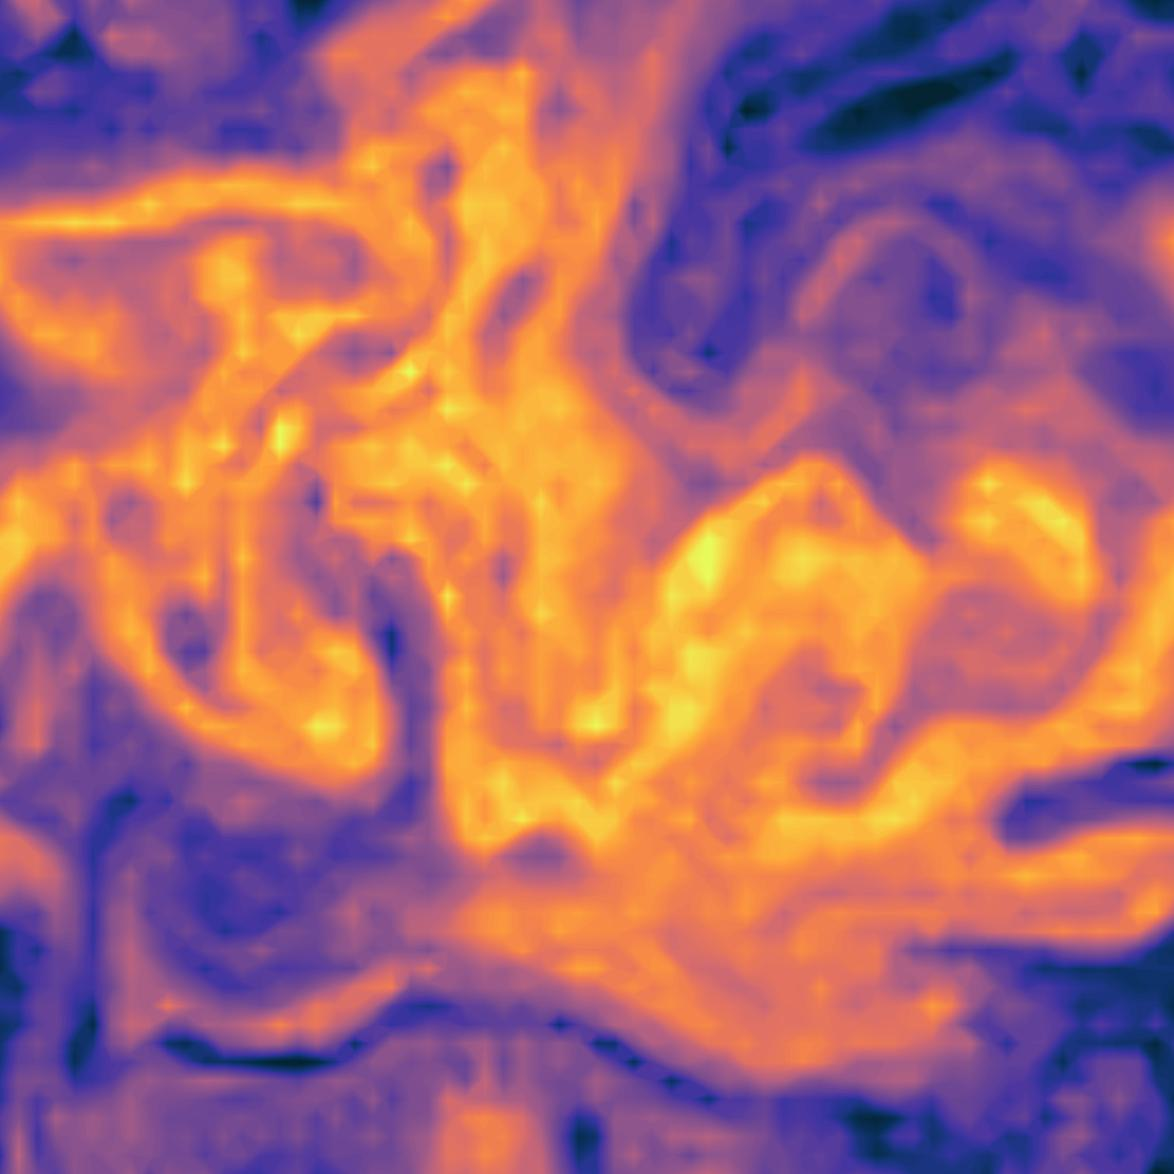
\includegraphics[width=.22\textwidth]{../../figures/theta-z0.jpg}
        };
        \node at
            ($ (t0.north) + (0.0, 0.5) $)
            {$\inputstate(t)$};

        \node(tp1) at (8, 6){
            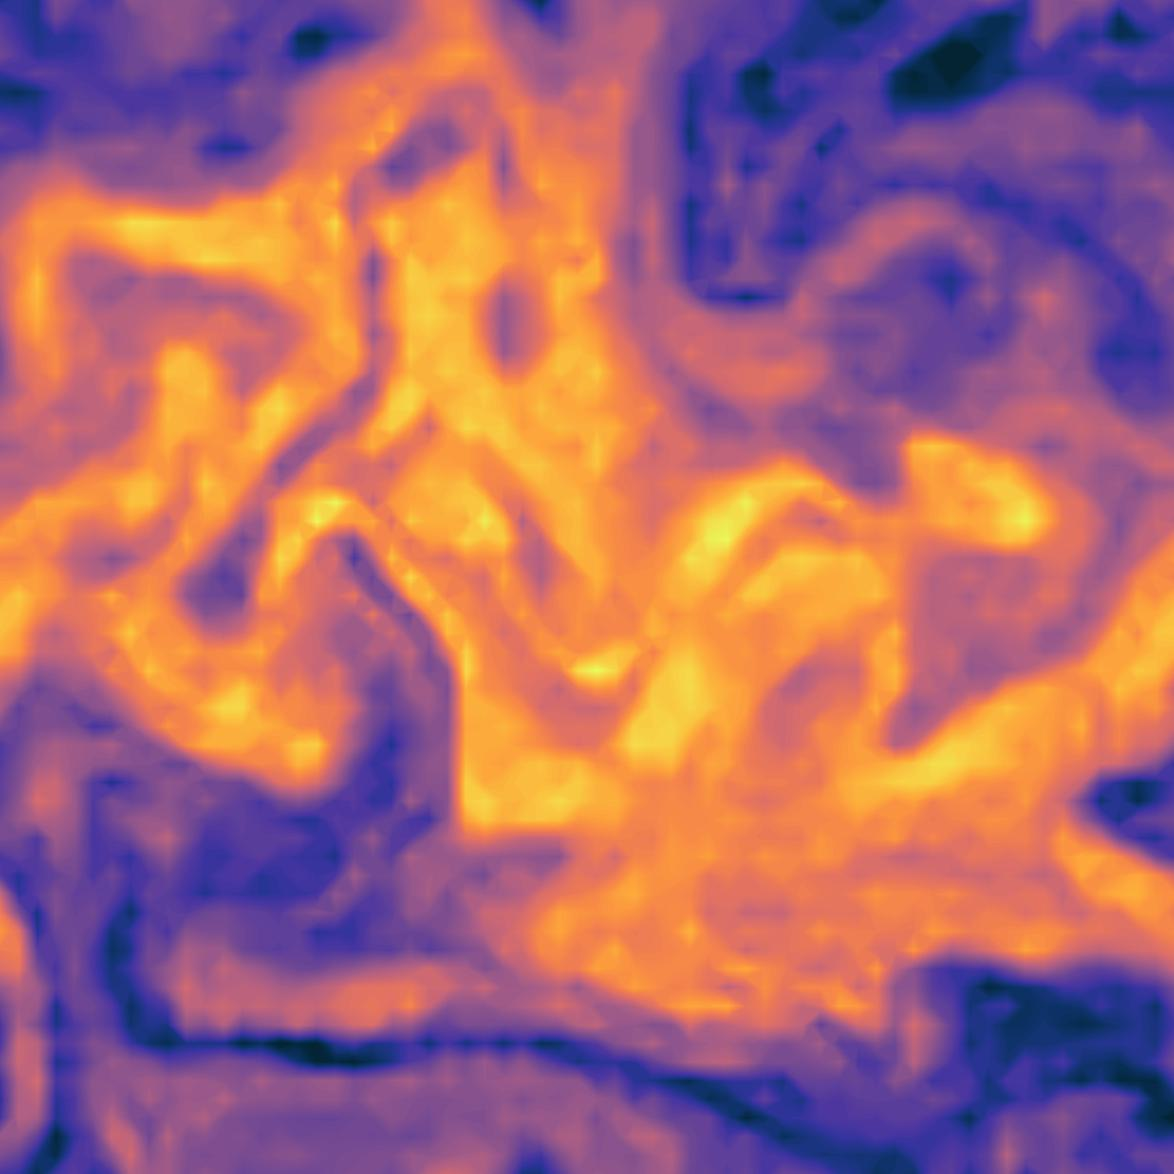
\includegraphics[width=.22\textwidth]{../../figures/theta-t1.jpg}
        };
        \node at
            ($ (tp1.north) + (0.0, 0.5) $)
            {$\inputstate(t+1)$};

        % --- RNN
        \node[rectangle,
            draw=black,
            minimum height=7.5em,
            minimum width=2em,
            line width=3pt,
            draw opacity=1,
            rounded corners=.5em] (rnn) at (8, -6) {};
        \node[circle,
            fill=sapphire,
            minimum height=0.5em,
            fill opacity=1] at (8, -3) {};
        \node[circle,
            fill=sapphire,
            minimum height=0.5em,
            fill opacity=1] at (8, -5) {};
        \node[circle,
            fill=sapphire,
            minimum height=0.5em,
            fill opacity=1] at (8, -7) {};
        \node[circle,
            fill=sapphire,
            minimum height=0.5em,
            fill opacity=1] at (8, -9) {};
        \node at
            ($ (rnn.south) - (0.0, 1.0) $) {$\hidden(t+1)$};

        % --- Connections
        \draw[line width=8pt, -{Stealth}, draw=gray]
            (t0.south) to [out=-90, in=-180] (rnn.west);
        \draw[line width=8pt, -{Stealth}, draw=gray]
            (tm1.south) to [out=-90, in=-180] (rnn.west);
        \draw[line width=8pt, -{Stealth}, draw=emerald]
            (rnn.north) to (tp1.south);

    \end{tikzpicture}
\end{minipage}


\vspace{-6em}
\begin{itemize}
    \item Build next\\hidden state, $\hidden(t+1)$,\\
        explicitly from input state at\\
        current and previous timesteps:\\
        $\{\inputstate(t), ..., \inputstate(t-N_\text{lag})\}$
    \item Here, consider quadratic relation between\\neighboring grid cells
    \item Map hidden state to target state
        \begin{equation*}
            \inputstate(t+1) = \textcolor{emerald}{\Wout} \hidden(t+1)
        \end{equation*}
        via trained readout matrix:
        \vspace{.5em}
        \begin{equation*}
            \Wout \coloneqq \argmin \left\{
                \dfrac{1}{2}\sum_{n=1}^{\ntrain} \norm{\Wout \hidden_n - \state_n}^2
                +
                \dfrac{\tikhonov}{2}\norm{\Wout}_\text{F}^2 \, \right\}
        \end{equation*}
    \item Note: hidden space is larger than input/target space
\end{itemize}

\begin{minipage}{\textwidth}
    \centering
    \begin{tikzpicture}[scale=1]

        % --- State vectors
        \node(tm1) at (-8, 0){
            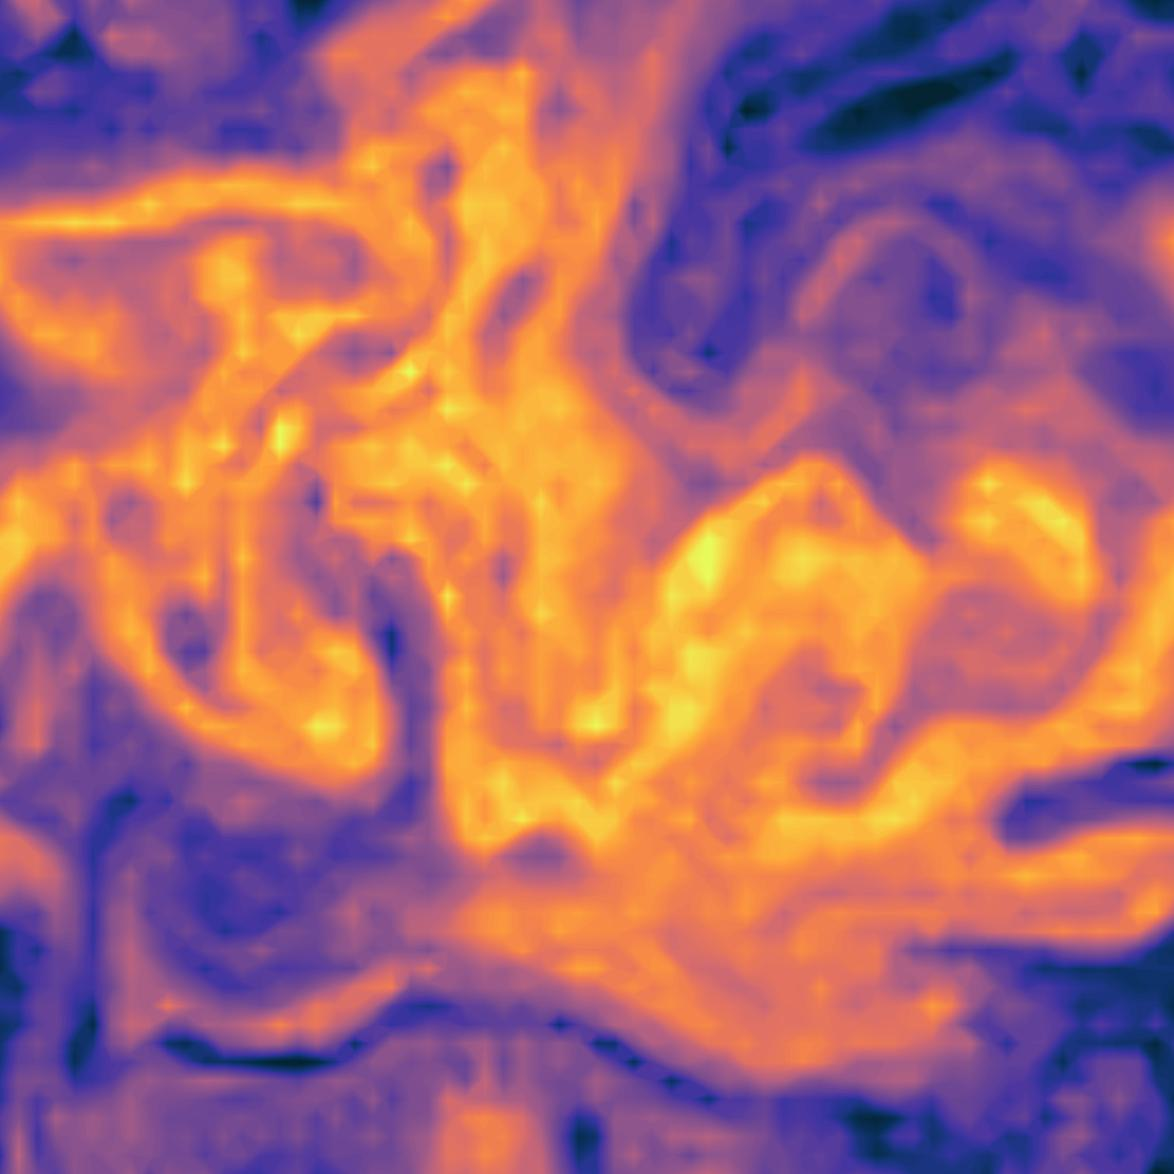
\includegraphics[width=.22\textwidth]{../../figures/theta-z0.jpg}
        };
        \node(tp1) at (8, 0){
            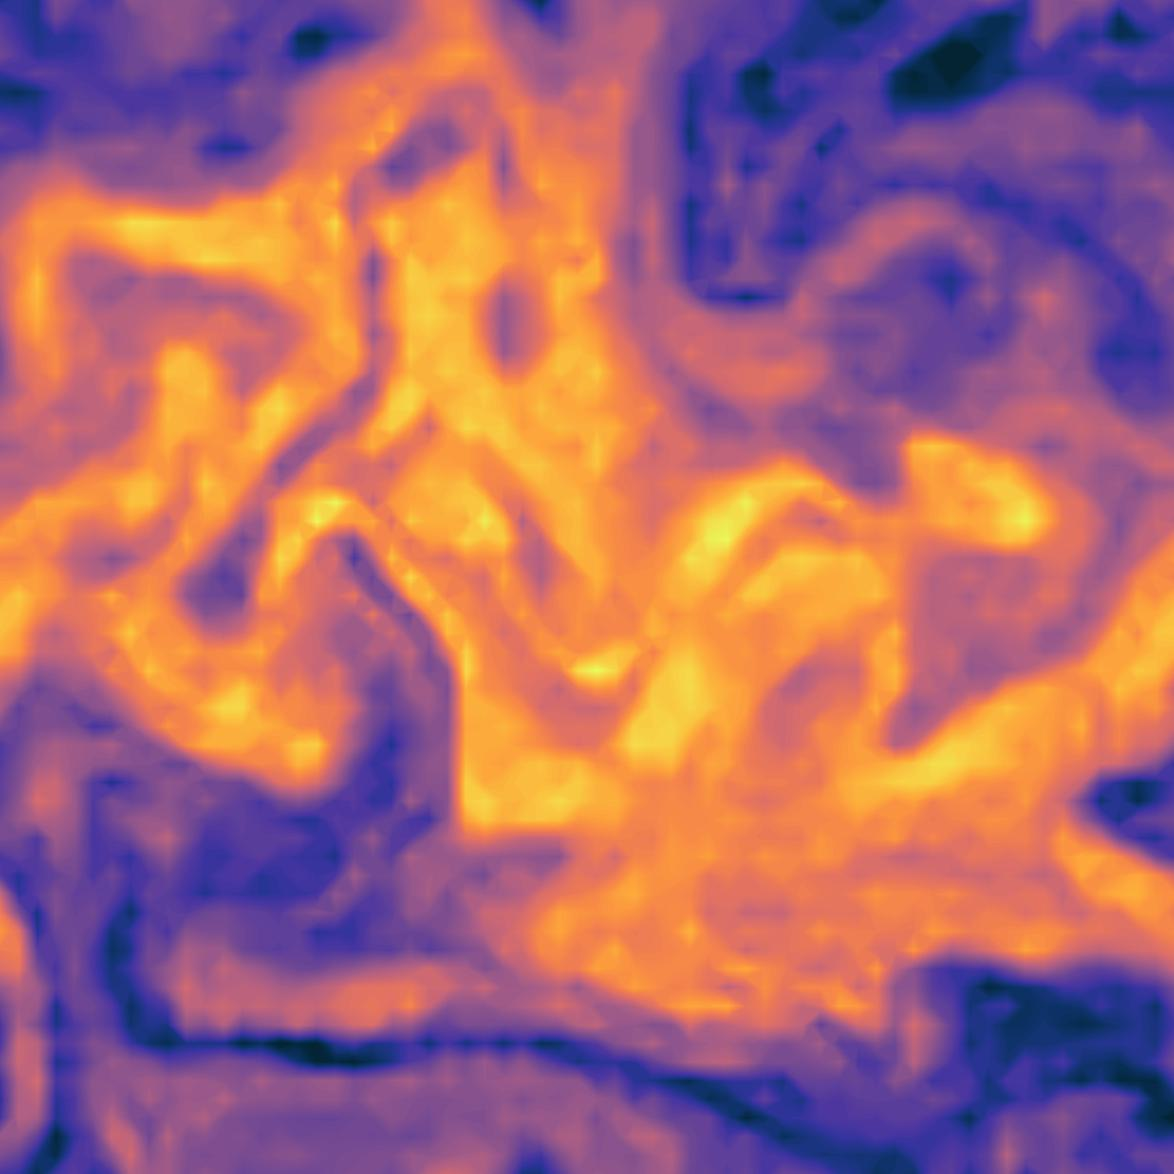
\includegraphics[width=.22\textwidth]{../../figures/theta-t1.jpg}
        };

        % --- RNN
        \node[rectangle,
            draw=black,
            minimum height=7.5em,
            minimum width=2em,
            line width=3pt,
            draw opacity=1,
            rounded corners=.5em] (rnn) at (0, 0) {};
        \node[circle,
            fill=sapphire,
            minimum height=0.5em,
            fill opacity=1] at (0, 3) {};
        \node[circle,
            fill=sapphire,
            minimum height=0.5em,
            fill opacity=1] at (0, 1) {};
        \node[circle,
            fill=sapphire,
            minimum height=0.5em,
            fill opacity=1] at (0, -1) {};
        \node[circle,
            fill=sapphire,
            minimum height=0.5em,
            fill opacity=1] at (0, -3) {};

        % --- Mappings
        \node[trapezium,
            fill=gray,
            fill opacity=1,
            minimum width=7.25em,
            minimum height=2em,
            trapezium angle=80,
            trapezium stretches=true,
            rotate=90] at (-3, 0) {};

        \node[trapezium,
            fill=emerald,
            fill opacity=1,
            minimum width=7.25em,
            minimum height=2em,
            trapezium angle=80,
            trapezium stretches=true,
            rotate=-90] at (3, 0) {};
    \end{tikzpicture}
\end{minipage}

\vspace{0.5em}
\hfill\begin{minipage}{0.97\textwidth}
    so we implement a parallization strategy akin to standard domain
    decomposition in GCMs
\end{minipage}

\section{Temporal Subsampling}

\vspace{.5em}
\begin{minipage}{\textwidth}
    \centering
    \begin{tikzpicture}[scale=1,
        thick/.style={line width=10pt},
        ]

        \draw[thick, draw] (t0) (-15, -1.5) to (-15, 1.5);
        \draw[thick, draw] (-10, -1.5) to (-10, 1.5);
        \draw[thick, draw] (-5, -1.5) to (-5, 1.5);
        \draw[thick, draw] (5, -1.5) to (5, 1.5);
        \draw[thick, draw] (10, -1.5) to (10, 1.5);

        \draw[thick, draw] (-13.75, -0.75) to (-13.75, 0.75);
        \draw[thick, draw] (-12.50, -0.75) to (-12.50, 0.75);
        \draw[thick, draw] (-11.25, -0.75) to (-11.25, 0.75);

        \draw[thick, draw] (-8.75, -0.75) to (-8.75, 0.75);
        \draw[thick, draw] (-7.50, -0.75) to (-7.50, 0.75);
        \draw[thick, draw] (-6.25, -0.75) to (-6.25, 0.75);

        \draw[thick, draw] (6.25, -0.75) to (6.25, 0.75);
        \draw[thick, draw] (7.50, -0.75) to (7.50, 0.75);
        \draw[thick, draw] (8.75, -0.75) to (8.75, 0.75);

        \draw[line width=6pt] (-15, 0) to (-2.5, 0) {};
        \draw[line width=6pt, -{Stealth}] (2.5, 0) to (13, 0) {};

        \node at (0,0) {$\bullet\,\,\bullet\,\,\bullet$};

        \node at (-15, -2.5) {$t_0$};
        \node at ( 10, -2.5) {$t$};
        \node at (  5, -2.5) {$t-1$};
        \node at (-4.5, -2.5) {$t-N_\text{lag}$};

        \draw[decorate,
            decoration={brace, amplitude=10pt, raise=4pt},
            line width=5pt] (-13.75, 1.0) to (-12.50, 1.0);
        \node at (-13.125, 2.5) {$\Delta t$};

        \draw[decorate,
            decoration={brace, amplitude=10pt, raise=8pt},
            line width=5pt] (-10, 1.6) to (-5, 1.6);
        \node at (-7.5, 3.25) {$N_\text{sub}\Delta t$};

    \end{tikzpicture}
\end{minipage}


\section{References}
\vspace{1em}
\begin{minipage}{\textwidth}
    \fontsizeinstitution
        \citeps{pathak_using_2017} doi: 10.1063/1.5010300 \\
        \citeps{platt_systematic_2022} doi: 10.1016/j.neunet.2022.06.025 \\
        \citeps{penny_integrating_2022} doi: 10.1029/2021MS002843 \\
        \citeps{tulloch_note_2009} doi: 10.1175/2008JAS2921.1 \\
        \citeps{zhang_catch-22_2022} doi: 10.48550/ARXIV.2210.10211
\end{minipage}
